\subsection{Systematiske test (white box test) (Magnus)}
\label{whitebox}

\subsubsection{Tilføj medarbejder til program}

Programmet er saniteret, så der ikke kan oprettes \texttt{Employee} objekter udenfor \texttt{App} klassen. Kun \texttt{App} har adgang til \texttt{Employee} contructoren, så nye medarbejdere oprettes og tilføjes ved:
\begin{enumerate}
\item gennem \texttt{app} objektet (instans af klassen \texttt{App}), køres metoden:  \\
    \texttt{public Employee newEmployee(String initials, String name)}
\item ovenstående metode  opretter et \texttt{Employee} objekt, og kører i \texttt{app}: \\
\texttt{private void addEmployee(Employee newEmp)}
\end{enumerate}

Det giver derfor mest mening at se disse metoder som helhed ved denne test.

\begin{lstlisting}
public Employee newEmployee(String initials, String name)
  throws NotUniqueInitialsException, InvalidEmployeeInitialsException, InvalidEmployeeNameException {

Employee employee = new Employee(initials, name);
addEmployee(employee);

return employee;
}

private void addEmployee(Employee newEmp) throws NotUniqueInitialsException {

for (Employee oldEmps : getEmployees()) { // 1
  if (oldEmps.getInitials().equals(newEmp.getInitials())) // 2
    throw new NotUniqueInitialsException();
}
  employees.add(newEmp); // 3
}
\end{lstlisting}

\begin{figure}[H]
    \centering
    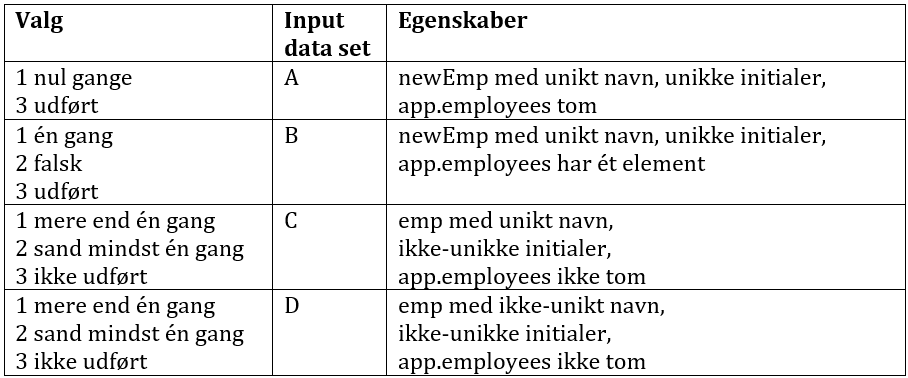
\includegraphics[width = \textwidth]{Figurer/whitebox1a.PNG}
    \label{fig:whitebox1a}
\end{figure}

Der refereres til følgende objekter i tabellen:
\begin{lstlisting}
Employee carl = app.newEmployee("cj", "Carl Janson");
Employee carl2 = app.newEmployee("cj", "Carl Janson");
\end{lstlisting}

\texttt{app.employees} er en \texttt{ArrayList}$<$\texttt{Employee}$>$ i \texttt{app}, der indeholder ingen elementer, eller:
\begin{lstlisting}
Employee susan = app.newEmployee("sb", "Susan Baker");
Employee caroline = app.newEmployee("cj", "Caroline Janson");
\end{lstlisting}

\begin{figure}[H]
    \centering
    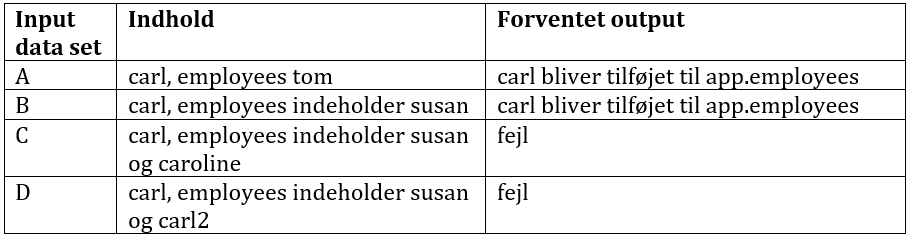
\includegraphics[width = \textwidth]{Figurer/whitebox1b.PNG}
    \label{fig:whitebox1b}
\end{figure}

Testkoden for de 4 tests er i \texttt{TestEmployeeNew.java}.

\begin{figure}[H]
    \centering
    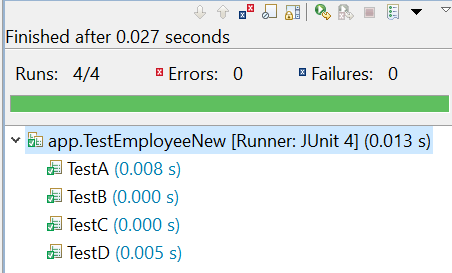
\includegraphics[width = 0.5 \textwidth]{Figurer/whitebox1succes.PNG}
    \caption{De 4 JUnit tests for "tilføj ny medarbejder" $\,$ har succes i Eclipse.}
    \label{fig:whitebox1succes}
\end{figure}




\subsubsection{Opret ny aktivitet i projekt}

Ligesom medarbejdere, oprettes nye aktiviteter kun gennem \texttt{app} objektet.
Konstruktøren til \texttt{Activity} er kun synlig for \texttt{app} objektet. \texttt{isActiveEmployee} er metode, der udfører yderligere condition checks for at afgøre, om den undersøgte bruger er aktiv (dvs. “logget ind”).

\begin{lstlisting}
public Activity newActivity(String name, Project project) throws Exception {

if (project == null) { // 1
  throw new Exception();
}
if (!isActiveEmployee(project.getProjectLeader())) // 2
  throw new NotProjectLeaderException();

Activity activity = new Activity(name, project);
project.addActivity(activity);

return activity;
  }
  
\end{lstlisting}


\begin{figure}[H]
    \centering
    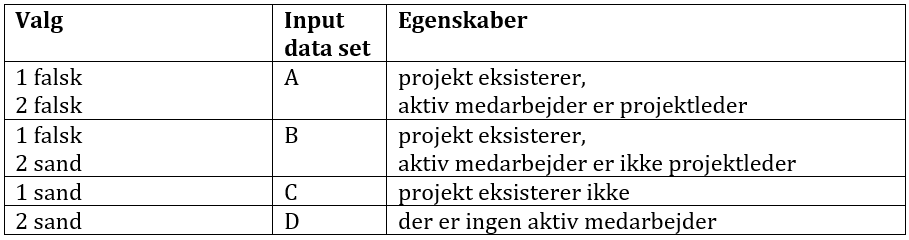
\includegraphics[width = \textwidth]{Figurer/whitebox2a.PNG}
    \label{fig:whitebox2a}
\end{figure}

Der refereres til følgende objekter i tabellen:
\begin{lstlisting}
Employee carl = app.newEmployee("cj", "Carl Janson");
Employee susan = app.newEmployee("sb", "Susan Baker");
Project master = app.newProject(carl, "Master Project", start, end);
Activity oprydning = app.newActivity("Oprydning", master);
\end{lstlisting}

samt \texttt{activeEmployee}, der er enten \texttt{null} (ingen medarbejder er aktiv), eller et \texttt{Employee}.

\begin{figure}[H]
    \centering
    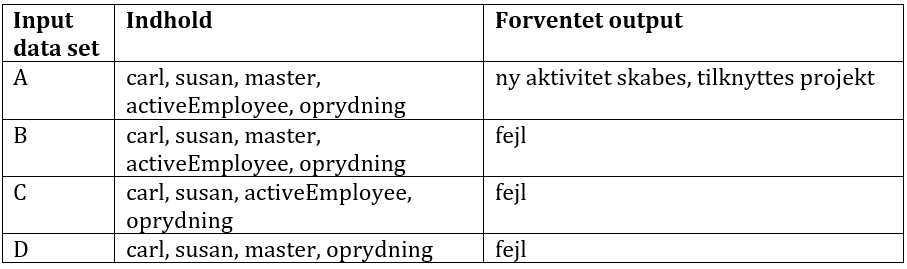
\includegraphics[width = \textwidth]{Figurer/whitebox2b.PNG}
    \label{fig:whitebox2b}
\end{figure}

Testkoden for de 4 tests er i \texttt{TestActivityNew.java}.

\begin{figure}[H]
    \centering
    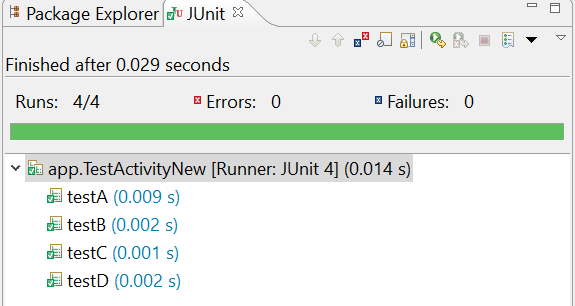
\includegraphics[width = 0.5 \textwidth]{Figurer/whitebox2succes.PNG}
    \caption{De 4 JUnit tests for "Opret ny aktivitet i projekt" $\,$ har succes i Eclipse.}
    \label{fig:whitebox2succes}
\end{figure}


\subsubsection{Opret ny statusaktivitet}
Det er værd at bemærke, at \texttt{Status} er implementeret som en enum med få mulige værdier. Dette reducerede antallet af condition checks i koden. 

\begin{lstlisting}
public StatusActivity newStatusActivity(Employee emp, Status status, String activityStart, String activityEnd)
  throws Exception {

if (emp == null) // 1
  throw new EmployeeNotFoundInAppException();

if (!isActiveEmployee(emp)) // 2
  throw new NotActiveEmployeeException();

StatusActivity sa = new StatusActivity(emp, status.toString(), status, activityStart, activityEnd);
addStatusActivity(sa);
emp.addActivity(sa);
return sa;
}
\end{lstlisting}

\begin{figure}[H]
    \centering
    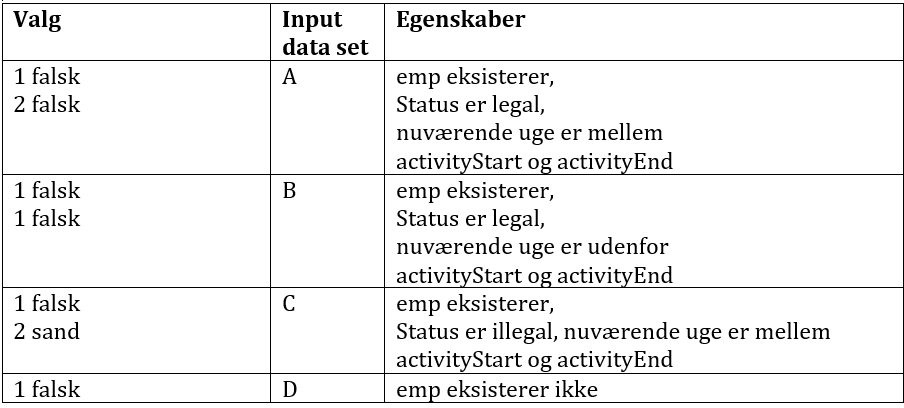
\includegraphics[width = \textwidth]{Figurer/whitebox3a.PNG}
    \label{fig:whitebox3a}
\end{figure}

\texttt{Status} er legal hvis den er defineret i enum \texttt{Status} og har værdien \texttt{SYG}, \texttt{FERIE}, eller \texttt{KURSUS}.

Der refereres til følgende objekter i tabellerne:
\begin{itemize}
\item \texttt{Employee carl = app.newEmployee("cj", "Carl Janson");} 
\item \texttt{sygNu}, som er en instans af \texttt{StatusActivity} hvis start- og sluttidspunkt indeholder den nuværende uge.
\item \texttt{sygSenere}, som er en instans af \texttt{StatusActivity} hvis start- og sluttidspunkt ikke indeholder den nuværende uge.
\item \texttt{doed}, som er en en \texttt{StatusActivity} med \texttt{Status.DOED}. 
\end{itemize}


\begin{figure}[H]
    \centering
    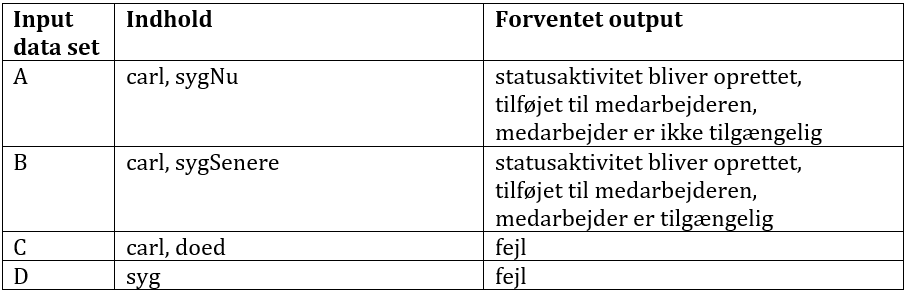
\includegraphics[width = \textwidth]{Figurer/whitebox3b.PNG}
    \label{fig:whitebox3b}
\end{figure}

Testkoden for de 4 tests er i  \texttt{TestActivityStatusNew.java}.

\begin{figure}[H]
    \centering
    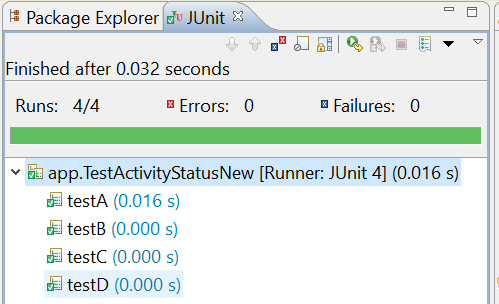
\includegraphics[width = 0.5 \textwidth]{Figurer/whitebox3succes.PNG}
    \caption{De 4 JUnit tests for "Opret ny statusaktivitet i projekt" $\,$ har succes i Eclipse.}
    \label{fig:whitebox3succes}
\end{figure}


\subsubsection{Tjek en medarbejders tilgængelighed}

Nær beslægtet med statusaktiviteter er en medarbejders tilgængelighed.
En medarbejder er utilgængelig, hvis han har en statusaktivitet, hvis start- og sluttidspunkt indeholder den nuværende uge. Eller hvis han har 20 eller flere  almindelige aktiviteter.

\begin{lstlisting}
    public boolean employeeIsAvailable(Employee emp) {

    for (StatusActivity sa : emp.getStatusActivities()) { // 1
      if (dateManager.currentDateIsBetween(sa.getActivityStart(), sa.getActivityEnd())) // 2
        return false;
    }

    if (emp.getActivities().size() >= 20) // 3
      return false;

    return true;
  }
\end{lstlisting}

\begin{figure}[H]
    \centering
    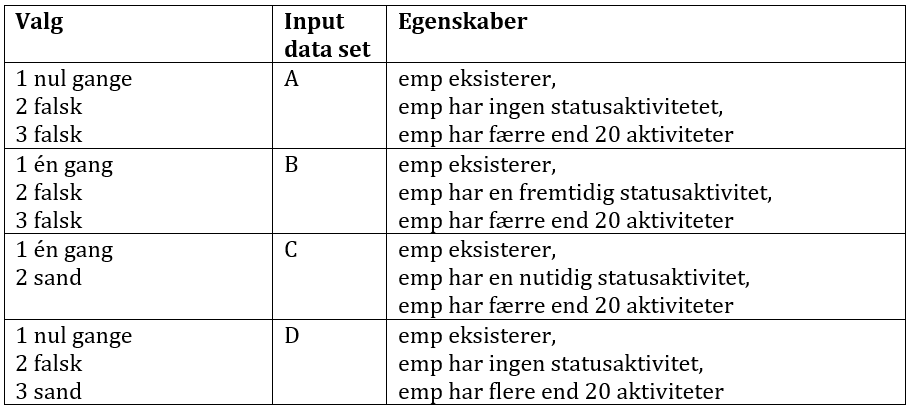
\includegraphics[width = \textwidth]{Figurer/whitebox4a.PNG}
    \label{fig:whitebox4a}
\end{figure}

I tabellerne refereres til objekterne:
\begin{lstlisting}
Employee carl = app.newEmployee("cj", "Carl Janson");
StatusActivity kursus = app.newStatusActivity(carl, Status.KURSUS, start, end); // fremtid
StatusActivity syg = app.newStatusActivity(carl, Status.SYG, start, end); // nutid
\end{lstlisting}

Samt 21 aktiviteter af typen \texttt{Activity}, tilknyttet \texttt{carl}.

\begin{figure}[H]
    \centering
    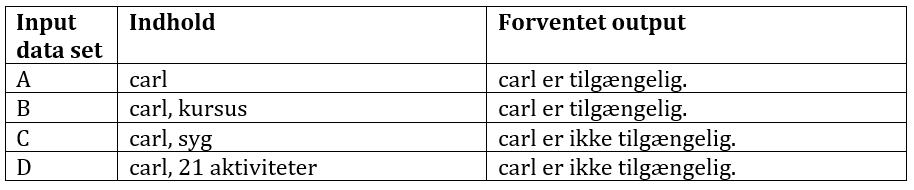
\includegraphics[width = \textwidth]{Figurer/whitebox4b.PNG}
    \label{fig:whitebox4b}
\end{figure}

Testkoden for de 4 tests er i \texttt{TestEmployeeIsAvailable.java}.

\begin{figure}[H]
    \centering
    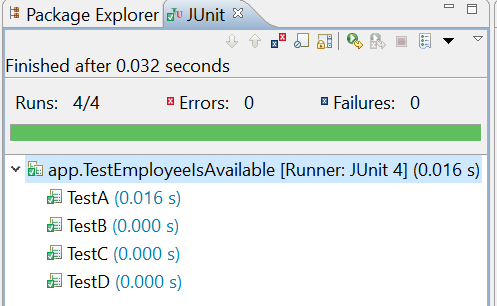
\includegraphics[width = 0.5 \textwidth]{Figurer/whitebox4succes.PNG}
    \caption{De 4 JUnit tests for "Tjek en medarbejders tilgængelighed" $\,$ har succes i Eclipse.}
    \label{fig:whitebox4succes}
\end{figure}